\documentclass[a4paper]{article}
%\usepackage[singlespacing]{setspace}
\usepackage[onehalfspacing]{setspace}
%\usepackage[doublespacing]{setspace}
\usepackage{geometry} % Required for adjusting page dimensions and margins
\usepackage{amsmath,amsfonts,stmaryrd,amssymb,mathtools,dsfont} % Math packages
\usepackage{tabularx}
\usepackage{colortbl}
\usepackage{listings}
\usepackage{amsmath}
\usepackage{amssymb}
\usepackage{amsthm}
\usepackage{subcaption}
\usepackage{float}
\usepackage[table,xcdraw]{xcolor}
\usepackage{tikz-qtree}
\usepackage{forest}
\usepackage{changepage,titlesec,fancyhdr} % For styling Header and Titles
\pagestyle{fancy}

\usepackage{enumerate} % Custom item numbers for enumerations

\usepackage[ruled]{algorithm2e} % Algorithms

\usepackage[framemethod=tikz]{mdframed} % Allows defining custom boxed/framed environments

\usepackage{listings} % File listings, with syntax highlighting
\lstset{
	basicstyle=\ttfamily, % Typeset listings in monospace font
}

\usepackage[ddmmyyyy]{datetime}


\geometry{
	paper=a4paper, % Paper size, change to letterpaper for US letter size
	top=2.5cm, % Top margin
	bottom=3cm, % Bottom margin
	left=2.5cm, % Left margin
	right=2.5cm, % Right margin
	headheight=25pt, % Header height
	footskip=1.5cm, % Space from the bottom margin to the baseline of the footer
	headsep=1cm, % Space from the top margin to the baseline of the header
	%showframe, % Uncomment to show how the type block is set on the page
}
\lhead{Stochastik für die Informatik\\Wintersemester 2024/2025}
\chead{\bfseries{Übungsblatt 1}\\}
\rhead{Lienkamp, 8128180\\Werner, 7987847}

\begin{document}

\setcounter{section}{1} % Setzt den Section-Zähler auf 1
\subsection{Inklusions-Exklusions-Formel}
Beweisen Sie die folgende Aussage für einen Wahrscheinlichkeitsraum $(\Omega, \mathbb{P})$:\\
Für beliebige Ereignisse $A_i \in \Omega, i = 1, 2, 3$ gilt\\\\
\(\mathbb{P}(A_1 \cup A_2 \cup A_3) = \left(\sum\limits^3_{i=1} \mathbb{P}(A_i)\right)-\mathbb{P}(A_1 \cap A_2) + \mathbb{P}(A_1 \cap A_3) - P(A_2 \cap A_3) + P(A_1 \cap A_2 \cap A_3)
\)\\\\
Gilt diese Aussage auch für die Kardinalität, d.h., gilt:\\\\
\(|A_1 \cup A_2 \cup A_3| = \sum\limits_{i=1}^{3} |A_i| - |A_1 \cap A_2| - |A_1 \cap A_3| - |A_2 \cap A_3| + |A_1 \cap A_2 \cap A_3|\)\\\\
für beliebige Ereignisse $A_i \subseteq \Omega$, $i = 1, 2, 3$?\\\\
\(\mathbb{P}(A_1 \cup A_2 \cup A_3)\\
\Rightarrow \mathbb{P}((A_1 \cup A_2) \cup A_3)\\
\Rightarrow \mathbb{P}(A_1 \cup A_2) + \mathbb{P}(A_3) - \mathbb{P}((A_1 \cup A_2) \cap A_3)\\
\Rightarrow \mathbb{P}(A_1) + \mathbb{P}(A_2) -\mathbb{P}(A_1 \cap A_2) + \mathbb{P}(A_3) - \mathbb{P}((A_1 \cup A_2) \cap A_3)\\
\Rightarrow \mathbb{P}(A_1) + \mathbb{P}(A_2) + \mathbb{P}(A_3) -\mathbb{P}(A_1 \cap A_2) - \mathbb{P}((A_1 \cup A_2) \cap A_3)\\
\Rightarrow \sum\limits_{i=1}^3\mathbb{P}(A_i) -\mathbb{P}(A_1 \cap A_2) - \mathbb{P}((A_1 \cup A_2) \cap A_3)\)\\
\textcolor{gray}{Nebenrechnung:\\
$\mathbb{P}(A_1\cup A_2)\cap A_3) \Rightarrow \mathbb{P}(A_1 \cap A_3)+\mathbb{P}(A_2 \cap A_3)-\mathbb{P}(A_1 \cap A_3 \cup A_2 \cap A_3) \\
\Rightarrow \mathbb{P}(A_1 \cap A_3) + \mathbb{P}(A_2 \cap A_3) - \mathbb{P}(A_1 \cap A_3 \cup A_2 \cap A_3)$\\
und $ (A_3 \cap A_3) = A_3$}\\
\(\Rightarrow \sum\limits_{i=1}^3\mathbb{P}(A_i) - ( \mathbb{P}(A_1 \cap A_3) + \mathbb{P}(A_2 \cap A_3) - \mathbb{P}(A_1 \cup A_2 \cap A_3))\\
\Rightarrow \sum\limits_{i=1}^3\mathbb{P}(A_i) - \mathbb{P}(A_1 \cap A_3) - \mathbb{P}(A_2 \cap A_3) + \mathbb{P}(A_1 \cup A_2 \cap A_3)\)\\\\
Die Aussage gilt auch für die Kardinalität, wenn gilt, dass $\vert A \cup B\vert = \vert A \vert + \vert B \vert - \vert A \cap B \vert$\\\\
\begin{tabular}{|l|l|l|l|}
    \hline
    Fall & $\vert A \cup B \vert$ & $\vert A \vert + \vert B \vert - \vert A \cap B \vert$ & $\triangle$\\
    \hline
    nur in A & $\vert 1 \cup 0 \vert = 1$ & $\vert 1 \vert + \vert 0 \vert - \vert 0 \vert = 1$ & $\triangle=0$\\
    \hline 
    nur in B & $\vert 0 \cup 1 \vert = 1$ & $\vert 0 \vert + \vert 1 \vert - \vert 0 \vert = 1$ & $\triangle=0$\\
    \hline in A und B & $\vert 1 \cup 1 \vert = 1$ & $\vert 1 \vert + \vert 1 \vert - \vert 1 \vert = 1$ & $\triangle=0$\\
    \hline 
\end{tabular}\\\\
Für Beweis siehe analog zum Wahrscheinlichkeitsraum.
\clearpage
\subsection{}
Eine Befragung von 1000 Personen im Rahmen einer Studie über Süßigkeiten ergab das folgende
Bild: 34 Personen mögen überhaupt keine Süßigkeiten, 803 Personen mögen Schokolade, 744
Bonbons, 400 Lollis, 571 Schokolade und Bonbons, 357 Schokolade und Lollis, 349 Bonbons und
Lollis sowie 297 Schokolade, Bonbons und Lollis. Begründen Sie, dass diese Zahlen einen Fehler
enthalten.\\
\textit{Hinweis: Verwenden Sie Aufgabe 1}
Wir verwenden die in \textit{1.1} bewiesene Aussage\\ 
\(|A_1 \cup A_2 \cup A_3| = \sum\limits_{i=1}^{3} |A_i| - |A_1 \cap A_2| - |A_1 \cap A_3| - |A_2 \cap A_3| + |A_1 \cap A_2 \cap A_3|\\
\Rightarrow 803 + 744 + 400 - 571 - 357 - 297 = 967 \neq 966 = 1000-34\)

\begin{center}
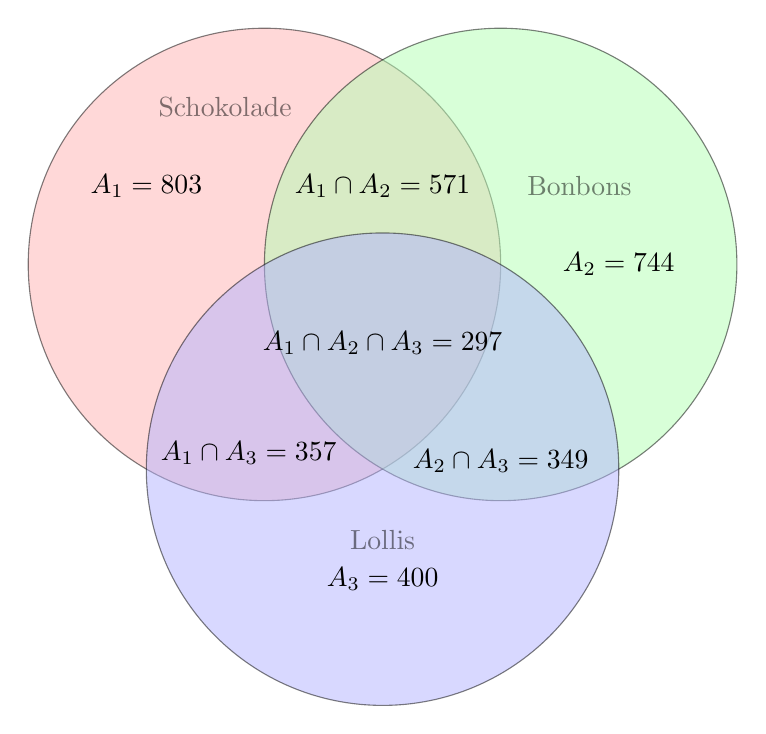
\begin{tikzpicture}[scale=2]
    % Draw the circles
    \draw[fill=red!30, opacity=0.5] (0,0) circle (1.5) node at (-0.25,1) {Schokolade};
    \draw[fill=green!30, opacity=0.5] (1.5,0) circle (1.5) node at (2, 0.5) {Bonbons};
    \draw[fill=blue!30, opacity=0.5] (0.75,-1.3) circle (1.5) node at (0.75,-1.75) {Lollis};

    % Label the intersections and unique parts
    % A only
    \node at (-0.75, 0.5) {$A_1 = 803$};
    % B only
    \node at (2.25, 0) {$A_2 = 744$};
    % C only
    \node at (0.75,-2.0) {$A_3 = 400$};
    
    % A ∩ B
    \node at (0.75, 0.5) {$A_1 \cap A_2 = 571$};
    % A ∩ C
    \node at (-0.1,-1.2) {$A_1 \cap A_3 = 357$};
    % B ∩ C
    \node at (1.5,-1.25) {$A_2 \cap A_3 = 349$};
    
    % A ∩ B ∩ C
    \node at (0.75,-0.5) {$A_1 \cap A_2 \cap A_3 = 297$};
\end{tikzpicture}\\
\[\sum\limits^3_{i=1}\lvert A_i \rvert - \lvert A_1 \cap A_2 \rvert - \lvert A_1 \cap A_3 \rvert - \lvert A_2 \cap A_3 \rvert + \lvert A_1 \cap A_2 \cap A_3 \rvert\]
\[\Rightarrow 803 + 744 + 400 - 571 - 357 - 349 + 297 = 967 \neq 966 = 1000 - 34\]
\end{center}
\clearpage
\subsection{Bedingte Wahrscheinlichkeiten}
Bei der 1. Klausur Stochastik für die Informatik in einem vorigen Jahr haben 168 Studierende
teilgenommen und davon 100 bestanden. Außerdem haben von den 168 Teilnehmern 88 Bonuspunkte bekommen (welche nicht zum Bestehen der Klausur beitragen können), indem sie mehr als 50\% der Hausaufgabenpunkte erreicht haben. Von den Studierenden, die Bonuspunkte erzielt haben, haben 65 die Klausur bestanden. Wir wählen nun zufällig einen Studenten aus und bezeichnen mit A das Ereignis, dass dieser Student die Klausur bestanden hat und mit B das Ereignis, dass er Bonuspunkte erzielt hat.\\
Berechnen Sie\\
a) $\mathbb{P}(A \mid B)$\\\\
\(\mathbb{P}(A\vert B) = \frac{65}{88}\) Aus Aufgabe abgelesen.\\\\
b) $\mathbb{P}(A \cup B)$\\\\
\(\mathbb{P}(A \cup B) = \mathbb{P}(A) + \mathbb{P}(B)- \mathbb{P}(A \cap B) \Rightarrow \frac{100}{168}+\frac{88}{168}-\frac{65}{168}=\frac{123}{168}=\frac{41}{56}\)\\
\textcolor{gray}{$\mathbb{P}(A \cap B) = \frac{65}{168}$}\\\\
c) $\mathbb{P}(A^c \cup B^c)$\\\\
\(\mathbb{P}(A^c \cup B^c)= \mathbb{P}(A^c)+ \mathbb{P}(B^c)- \mathbb{P}(A^c \cap B^c) \Rightarrow \frac{68}{168}+ \frac{80}{168}-\frac{45}{168}=\frac{103}{168}\)\\\\
d) $\mathbb{P}(A^c \mid B)$\\\\
\(\mathbb{P}(A^c\vert B) = \frac{23}{88}\) Aus Text abgelesen.\\\\
e) $\mathbb{P}(B^c \mid A^c)$\\\\
\(\mathbb{P}(B^c\vert A^c)=\frac{\mathbb{P}(A^c \cap B^c)}{\mathbb{P}(A^c)}\Rightarrow \frac{45}{168}:\frac{68}{168}= \frac{45}{168}\cdot \frac{168}{68}=\frac{45}{68}\)

\begin{center}
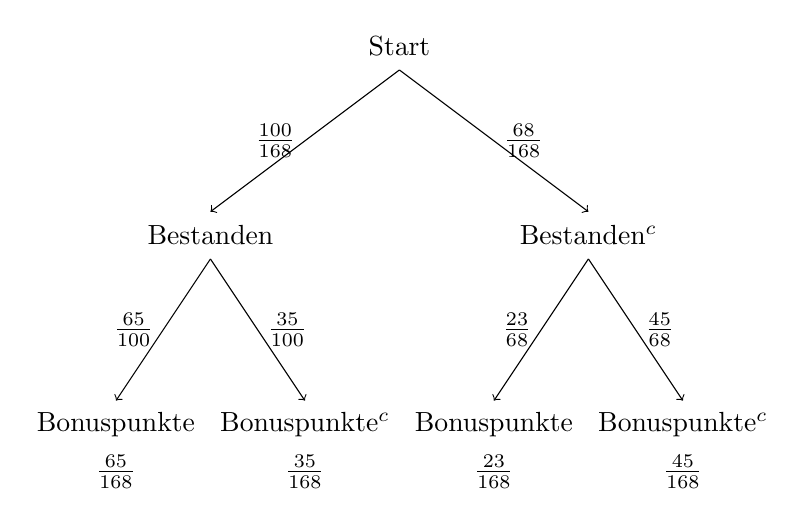
\begin{tikzpicture}[scale=1.2]

    % Draw the root
    \node at (0,0) {Start};
    
    % First level
    \node at (-2,-2) {Bestanden};
    \node at (2,-2) {Bestanden$^c$};
    
    % Second level
    \node at (-3,-4) {Bonuspunkte};
    \node at (-1,-4) {Bonuspunkte$^c$};
    
    \node at (1,-4) {Bonuspunkte};
    \node at (3,-4) {Bonuspunkte$^c$};
    
    % End probabilities
    \node at (-3,-4.5) {\(\frac{65}{168}\)};
    \node at (-1,-4.5) {\(\frac{35}{168}\)};
    \node at (1,-4.5) {\(\frac{23}{168}\)};
    \node at (3,-4.5) {\(\frac{45}{168}\)};
    
    % Draw the branches with probabilities as proper fractions
    \draw[->] (0,-0.25) -- (-2,-1.75) node[midway, left] {\(\frac{100}{168}\)};
    \draw[->] (0,-0.25) -- (2,-1.75) node[midway, right] {\(\frac{68}{168}\)};
    
    \draw[->] (-2,-2.25) -- (-3,-3.75) node[midway, left] {\(\frac{65}{100}\)};
    \draw[->] (-2,-2.25) -- (-1,-3.75) node[midway, right] {\(\frac{35}{100}\)};
    
    \draw[->] (2,-2.25) -- (1,-3.75) node[midway, left] {\(\frac{23}{68}\)};
    \draw[->] (2,-2.25) -- (3,-3.75) node[midway, right] {\(\frac{45}{68}\)};
    
\end{tikzpicture}
\end{center}
\clearpage
\subsection{Bedingte Wahrscheinlichkeiten}
Eine Urne enthält sechs schwarze und vier weiße Kugeln, eine zweite Urne enthält fünf schwarze
und fünf weiße Kugeln. Eine faire Münze wird geworfen um zu entscheiden, aus welcher Urne
gezogen wird. Man zieht dann nacheinander mit Zurücklegen zwei Kugeln aus der gewählten
Urne.\\\\
\begin{center}
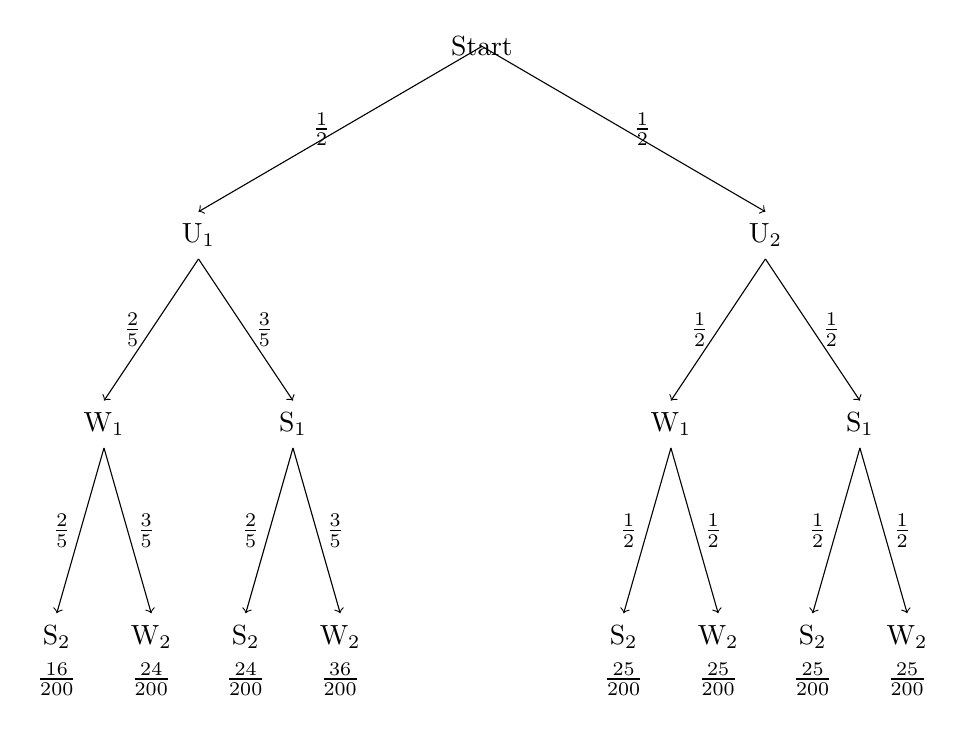
\begin{tikzpicture}[scale=1.2, every node/.style={align=center}]

    % Draw the root
    \node at (0,0) {Start};

    % First level
    \node at (-3,-2) {U$_1$};
    \node at (3,-2) {U$_2$};

    % Second level
    \node at (-4,-4) {W$_1$};
    \node at (-2,-4) {S$_1$};

    \node at (2,-4) {W$_1$};
    \node at (4,-4) {S$_1$};

    % Third level for W1 and S1
    \node at (-4.5,-6.5) {S$_2$ \\ \(\frac{16}{200}\)};
    \node at (-3.5,-6.5) {W$_2$ \\ \(\frac{24}{200}\)};
    
    \node at (-2.5,-6.5) {S$_2$ \\ \(\frac{24}{200}\)};
    \node at (-1.5,-6.5) {W$_2$ \\ \(\frac{36}{200}\)};

    % Third level for S1
    \node at (1.5,-6.5) {S$_2$ \\ \(\frac{25}{200}\)};
    \node at (2.5,-6.5) {W$_2$ \\ \(\frac{25}{200}\)};

    \node at (3.5,-6.5) {S$_2$ \\ \(\frac{25}{200}\)};
    \node at (4.5,-6.5) {W$_2$ \\ \(\frac{25}{200}\)};

    % Draw the branches with probabilities
    \draw[->] (0,0) -- (-3,-1.75) node[midway, left] {\(\frac{1}{2}\)};
    \draw[->] (0,0) -- (3,-1.75) node[midway, right] {\(\frac{1}{2}\)};
    
    \draw[->] (-3,-2.25) -- (-4,-3.75) node[midway, left] {\(\frac{2}{5}\)};
    \draw[->] (-3,-2.25) -- (-2,-3.75) node[midway, right] {\(\frac{3}{5}\)};
    
    \draw[->] (3,-2.25) -- (2,-3.75) node[midway, left] {\(\frac{1}{2}\)};
    \draw[->] (3,-2.25) -- (4,-3.75) node[midway, right] {\(\frac{1}{2}\)};
    
    % Draw branches for W1
    \draw[->] (-4,-4.25) -- (-4.5,-6) node[midway, left] {\(\frac{2}{5}\)};
    \draw[->] (-4,-4.25) -- (-3.5,-6) node[midway, right] {\(\frac{3}{5}\)};
    
    % Draw branches for S1
    \draw[->] (-2,-4.25) -- (-2.5,-6) node[midway, left] {\(\frac{2}{5}\)};
    \draw[->] (-2,-4.25) -- (-1.5,-6) node[midway, right] {\(\frac{3}{5}\)};

    % Draw branches for U2
    \draw[->] (2,-4.25) -- (1.5,-6) node[midway, left] {\(\frac{1}{2}\)};
    \draw[->] (2,-4.25) -- (2.5,-6) node[midway, right] {\(\frac{1}{2}\)};
    
    \draw[->] (4,-4.25) -- (3.5,-6) node[midway, left] {\(\frac{1}{2}\)};
    \draw[->] (4,-4.25) -- (4.5,-6) node[midway, right] {\(\frac{1}{2}\)};

\end{tikzpicture}
\end{center}
(a) Wie groß ist die Wahrscheinlichkeit, dass die zweite Kugel schwarz ist?\\\\
Wir addieren alle Ergebnisse für eine schwarze Kugel, die im zweiten Zug gezogen wurde:\\
\(\frac{24}{200}+\frac{36}{200}+\frac{25}{200}+\frac{25}{200}=\frac{110}{200}=\frac{11}{20}\)\\\\
(b) Wie groß die Wahrscheinlichkeit, dass die zweite Kugel schwarz ist, falls die erste Kugel schwarz ist?\\\\
Wir berechnen zunächst die Wahrscheinlichkeiten der einzelnen Urnen (Urne wird gewählt($U_1/U_2$)), die erste Kugel ist schwarz($S_1)$, die zweite Kugel ist schwarz($S_2$) wir nennen diese Wahrscheinlichkeit $\mathbb{P}(A)$.\\
\(\mathbb{P}(U_1 \cap S_1 \cap S_2)= \frac{1}{2}\cdot\frac{3}{5}\cdot\frac{3}{5}=\frac{9}{50}\\
\mathbb{P}(U_2 \cap S_1 \cap S_2)= \frac{1}{2}\cdot\frac{1}{2}\cdot\frac{1}{2}= \frac{1}{8}\\
\mathbb{P}(U_1 \cap S_1 \cap S_2)\cup\mathbb{P}(U_2 \cap S_1 \cap S_2)\\
= \mathbb{P}(U_1 \cap S_1 \cap S_2) + \mathbb{P}(U_2 \cap S_1 \cap S_2) - \mathbb{P}(U_1 \cap S_1 \cap S_2)\cap\mathbb{P}(U_2 \cap S_1 \cap S_2)= \frac{36}{200}+\frac{25}{200}-0=\frac{61}{200} = \mathbb{P}(A)\)\\\\
Dann berechnen wir die Bedingung, dass eine schwarze Kugel gezogen wird unter der Bedingung, dass die erste Kugel auch schwarz war $\mathbb{P}(A)$(siehe (a))\\
\(\mathbb{P}(B \vert A) = \frac{\mathbb{P}(A \cap B)}{\mathbb{P}(A)}= \frac{61}{200} : \frac{11}{20}=\frac{122}{220}= \frac{61}{110}\)\\\\
\clearpage
\noindent (c) Wie groß die Wahrscheinlichkeit, dass die zweite Kugel schwarz ist, falls die Urne mit sechs schwarzen Kugeln gewählt wurde und die erste Kugel schwarz ist?\\\\
Da die Urne schon gewählt wurde und die erste schwarze Kugel bereits gezogen wurde, kann die Wahrscheinlichkeit mit $\frac{3}{5}$ aus dem Baum abgelesen werden.\\\\
(d) Wir betrachten die Ereignisse:\\
\hspace*{0,5cm}\textit{A}: die Urne mit sechs schwarzen Kugeln wird gewählt und die erste Kugel ist schwarz,\\
\hspace*{0,5cm}\textit{B}: die zweite Kugel ist schwarz\\
\hspace*{0,5cm}Berechnen Sie $\mathbb{P}(A), \mathbb{P}(B), \mathbb{P}(A \cap B)$\\\\
\(\mathbb{P}(A)=\mathbb{P}(U_1 \cap S_1)=\frac{1}{2}\cdot \frac{3}{5}=\frac{3}{10}\)\\
\(\mathbb{P}(B)=\frac{24}{200}+\frac{36}{200}+\frac{25}{200}+\frac{25}{200}=\frac{110}{200}=\frac{11}{20}\) (siehe (a))\\
\(\mathbb{P}(A \cap B)=\mathbb{P}(U_1 \cap S_1 \cap S_2)= \frac{1}{2}\cdot\frac{3}{5}\cdot\frac{3}{5}=\frac{9}{50}\) (siehe (c))
\end{document}
